\documentclass[9pt]{beamer}
\usetheme[progressbar=frametitle]{metropolis}

% Packages
\usepackage{appendixnumberbeamer}
\usepackage{booktabs}
\usepackage[scale=2]{ccicons}
\usepackage{graphicx}
\usepackage{amsmath}
\usepackage[font=tiny,skip=2pt]{caption}
\usepackage{subcaption}
\usepackage{xcolor}

\usepackage{siunitx}
\sisetup{
  detect-weight=true,
  detect-family=true,
  table-number-alignment = center,
  table-format=3.6,
  table-space-text-post = **
}

% Customize caption and table spacing for Beamer slides
\makeatletter
\AtBeginDocument{%
  \setbeamerfont{caption}{size=\tiny}
  \setbeamerfont{caption name}{size=\tiny}
  \setlength{\abovecaptionskip}{1pt}
  \setlength{\belowcaptionskip}{1pt}
  \renewenvironment{table}[1][]{%
    \def\@captype{table}%
    \par\vspace{0.15em}%
    \centering
  }{%
    \par\vspace{0.15em}%
  }%
}
\makeatother

% Title Info
\title{\Huge Modelling \& Forecasting\\Spanish Real GDP Growth}
\subtitle{Econometrics 20203 - Problem Set 2}
\author{Stefano Graziosi - 3174891 \\
        Gabriele Biroli - 3165990 \\
        Luca Gritti
        }
\institute{MSc Economic and Social Sciences, Università Bocconi}
\date{\today}

\begin{document}

\maketitle

% ============================================================
% SLIDE 1: Spain's GDP Growth History & Phases
% ============================================================
\begin{frame}{Spain's Real GDP Growth History \& Phases (1961--2025)}
\label{slide:history}
\begin{block}{}
\footnotesize
The series displays the expected post-war Spanish business-cycle features, with three main phases:
\end{block}

\begin{columns}

  \begin{column}{0.55\textwidth}
    \centering
    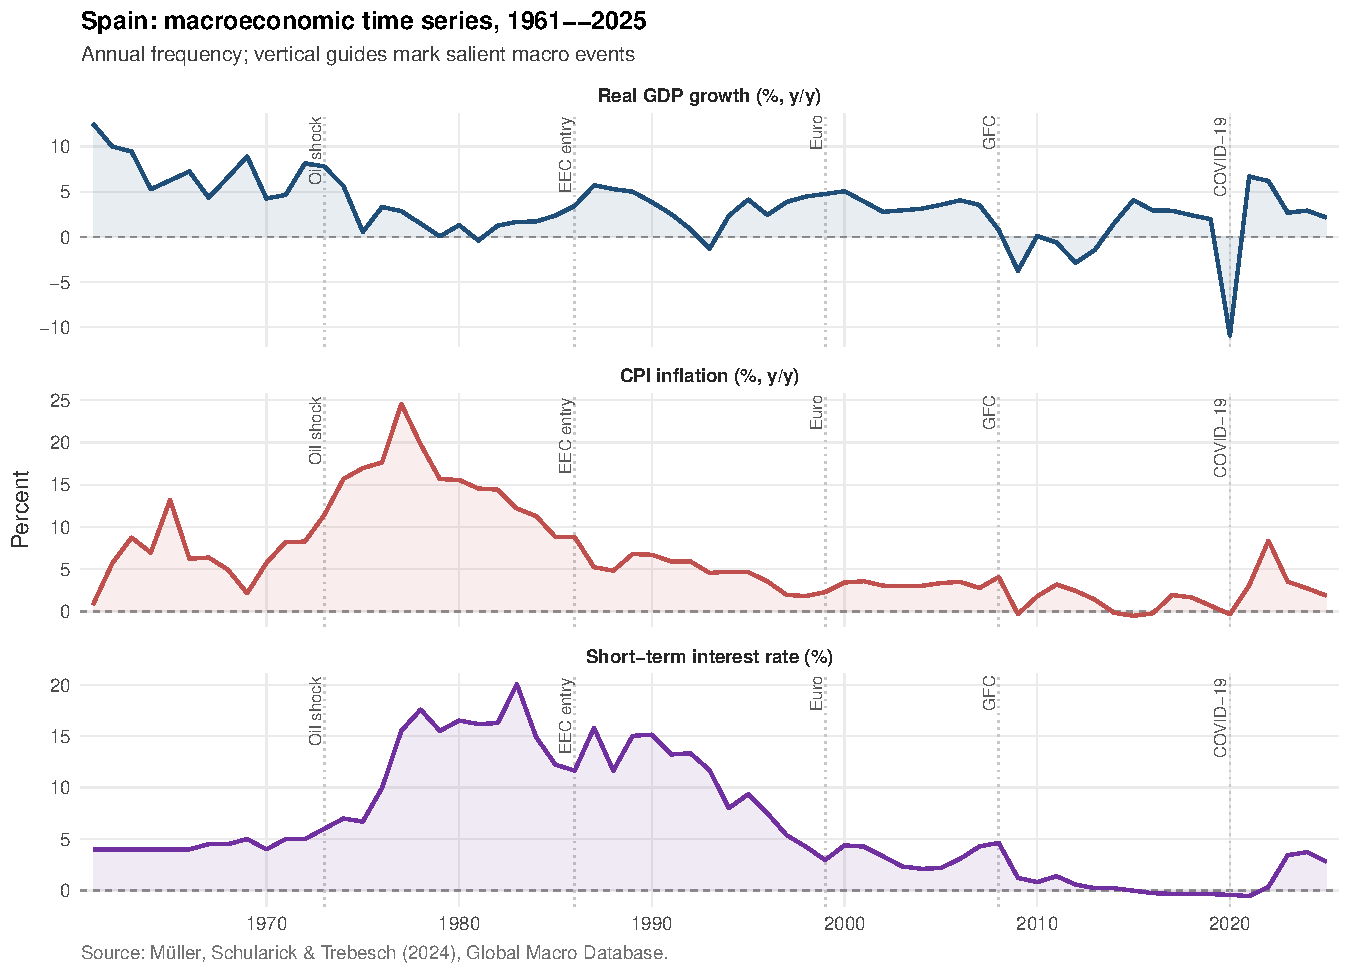
\includegraphics[width=\linewidth]{../output/figures/descriptive_plots.pdf}
  \end{column}

  \begin{column}{0.45\textwidth}
    \scriptsize
    \begin{itemize}
      \item \textbf{1961--2007:} GDP growth is centered around three percent on average, displaying the strong expansion of the Spanish miracle years and the post-EEC-accession boom, with broadly stable volatility of $\sim$2 pp.
      \item \textbf{2008--2013:} Two pronounced contractions define this period : the Global Financial Crisis (2008--09) and the subsequent euro-area sovereign-debt crisis (2011--13), pushing growth to sharply negative territory.
      \item \textbf{2014--2025:} A gradual recovery followed, then interrupted by the COVID-19 collapse of 2020 (-10.9 percent). The post-2021 energy shock is also visible in the accompanying inflation and interest-rate series. By 2023--25, growth has returned to a moderate positive path.
    \end{itemize}
  \end{column}

\end{columns}

\end{frame}


% ============================================================
% SLIDE 2: Dataset Composition
% ============================================================
\begin{frame}{Dataset Composition}
\label{slide:dataset}
\footnotesize

We work with annual observations from the \textbf{Global Macroeconomic Database} (Müller, Schularick, and Trebesch, 2024), which provides harmonised long series for real GDP, CPI inflation, and a short-term interest rate. We restrict the sample to \textbf{1960--2025} to focus on the modern, post-Bretton-Woods Spanish economy, avoiding structural breaks associated with the two World Wars, the Spanish Civil War (1936--39), and Franco-era autarky (1939--59). The resulting sample provides \textbf{65 year-on-year growth observations}, sufficient for all models considered.

\vspace{0.25cm}

The three variables entering the analysis are:
\begin{itemize}
  \item \textbf{Real GDP growth} \,($\Delta y_t$, \%)\,: target variable. Year-on-year percent change $100 \cdot (Y_t/Y_{t-1}-1)$. Captures Spain's output dynamics we wish to forecast.

  \item \textbf{CPI Inflation} \,($\pi_t$, \%)\,: demand-pressure and monetary-stance indicator. Rises sharply in the 1970s, moderates after EEC accession (1986) and euro adoption (1999); post-2021 energy shock briefly pushes it back above 8\%. Strongly correlated with the short rate (Taylor-rule relationship).

  \item \textbf{Short-term nominal interest rate} \,($i_t$, \%)\,: monetary-policy channel. Tracks the inflation pattern, declining from double digits in the 1980s to negative ECB-policy territory (2014--21) and rising again in 2023--25. Cross-correlation analysis shows short-rate movements lead GDP growth at horizons of 1--3 years, pointing to a monetary policy propagation mechanism.
\end{itemize}

\end{frame}


% ============================================================
% SLIDE 3: Descriptive Statistics
% ============================================================
\begin{frame}{Descriptive Statistics}
\label{slide:descriptive}

{\footnotesize
\setlength{\tabcolsep}{4pt}
\begin{table}

\caption{\label{tab:summary-stats}Summary statistics, 1961--2025}
\centering
\begin{tabular}[t]{lrrrrrrrr}
\toprule
Variable & N & Mean & Std. dev. & Min & Median & Max & Skewness & Kurtosis\\
\midrule
GDP growth (\%) & 65 & 3.24 & 3.46 & -10.94 & 3.11 & 12.54 & -0.70 & 6.42\\
Inflation (\%) & 65 & 6.23 & 5.49 & -0.50 & 4.67 & 24.54 & 1.20 & 3.89\\
Short rate (\%) & 65 & 6.38 & 5.67 & -0.55 & 4.28 & 20.05 & 0.73 & 2.24\\
\bottomrule
\end{tabular}
\end{table}

}

{\footnotesize
\begin{itemize}
    \item \textbf{GDP growth} has heavy left-tail behaviour (negative skew of $-0.70$ and kurtosis of $6.42$, well above the Gaussian value of three) driven by the GFC and COVID outliers. The mean of 3.24\% and SD of 3.46 reflect a moderately volatile series centred on moderate growth.

    \item \textbf{Inflation} is right-skewed (1.20) with a maximum of 24.54\%, reflecting the high-inflation episodes of the 1970s and early 1980s. Its wide range (nearly 25 pp) underlines the fundamental structural change in Spanish monetary conditions since EEC accession.

    \item \textbf{Short rate} mirrors the inflation pattern in skewness and range, consistent with a Taylor-rule-style policy reaction. The minimum of -0.55\% reflects the ECB's negative-rate policy window of 2014--21.
\end{itemize}
}

\end{frame}


% ============================================================
% SLIDE 4: Marginal Distributions & Bivariate Structure
% ============================================================
\begin{frame}{Marginal Distributions \& Bivariate Structure}
\label{slide:distributions}
\footnotesize
\begin{block}{}
\begin{columns}
  \begin{column}{0.5\textwidth}
    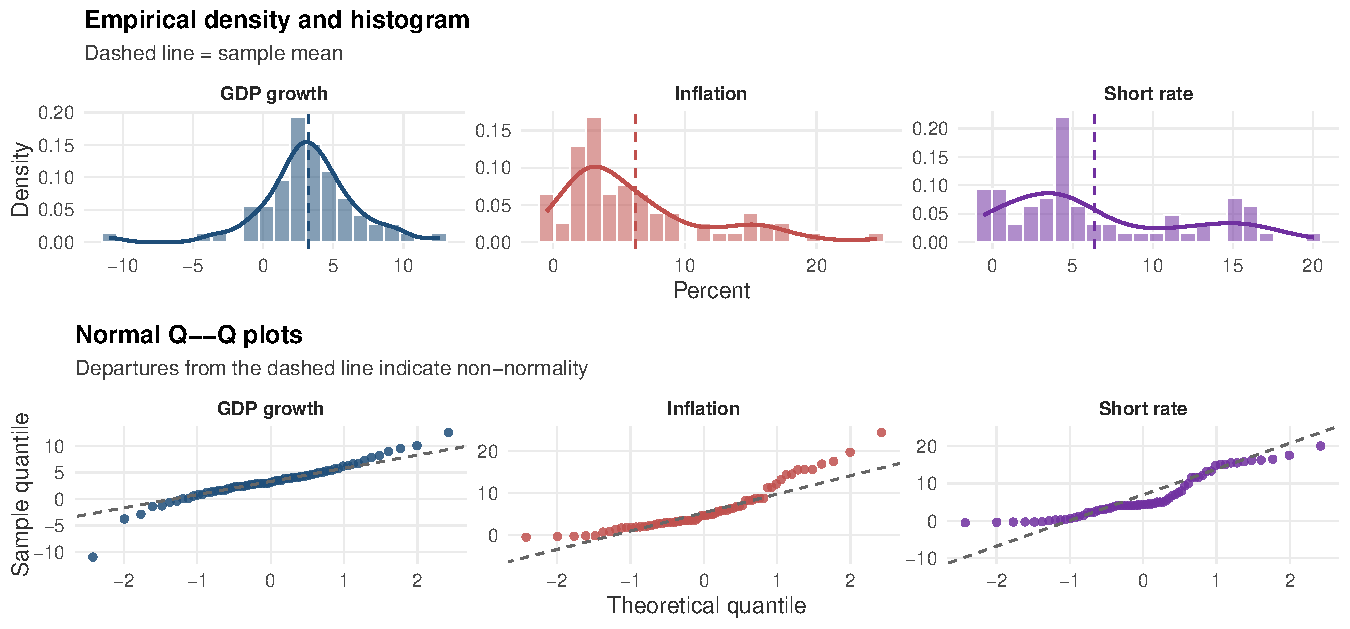
\includegraphics[width=\linewidth]{../output/figures/distribution_plots.pdf}
  \end{column}
  \begin{column}{0.5\textwidth}
    The histograms confirm the asymmetries already revealed by skewness and kurtosis: GDP growth has a long, thin left tail (GFC and COVID episodes) and a right-skewed inflation distribution dominated by the 1970s. The Q–Q plots display systematic deviations from normality, particularly in the tails; as we will see in Slide~\ref{slide:diagnostics}, the formal residual-normality tests confirm that this is mainly driven by extreme observations such as COVID.
  \end{column}
\end{columns}
\end{block}

\vspace{0.3cm}

\begin{block}{}
\begin{columns}
  \begin{column}{0.5\textwidth}
    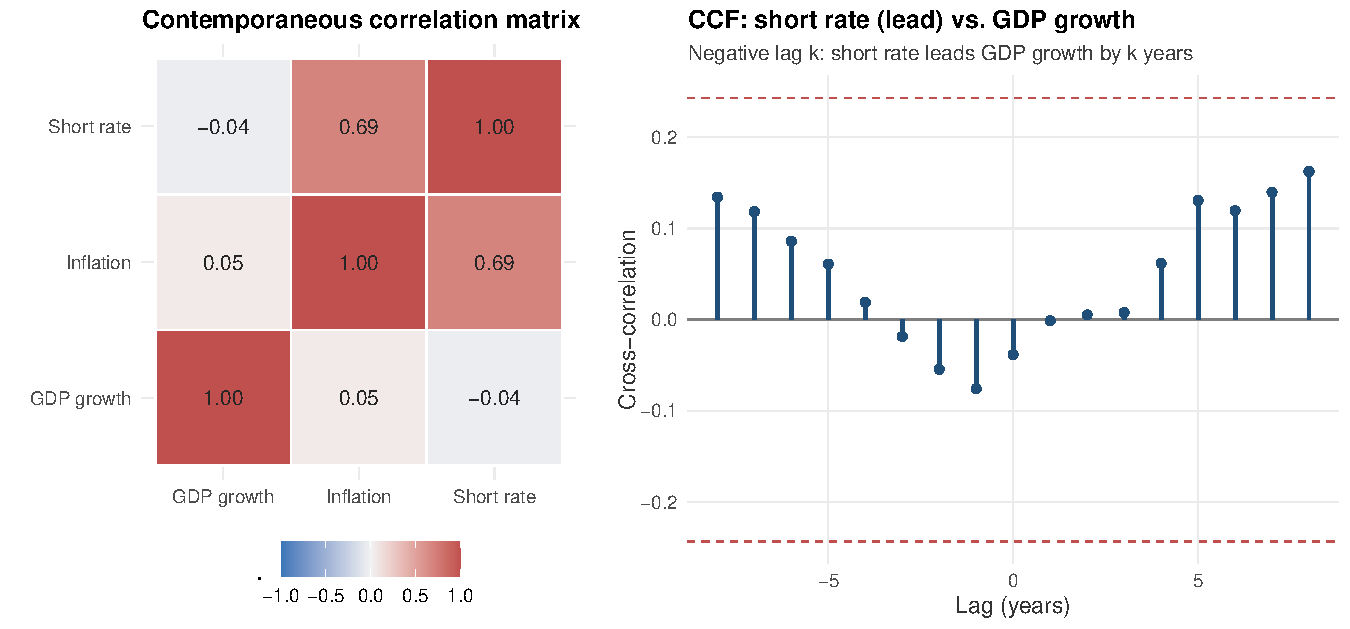
\includegraphics[width=\linewidth]{../output/figures/scatter_corr.pdf}
  \end{column}
  \begin{column}{0.5\textwidth}
    The contemporaneous correlation between GDP growth and the short rate is mildly negative, while inflation and the short rate are strongly positively correlated, consistent with a Taylor-rule-style policy reaction. The cross-correlation function shows that short-rate movements lead GDP growth at horizons of 1–3 years with a meaningful negative lead-correlation, pointing to a monetary policy propagation mechanism that we revisit in the impulse-response analysis on Slide~\ref{slide:granger-irf}.
  \end{column}
\end{columns}
\end{block}
\end{frame}


% ============================================================
% SLIDE 5: Rolling-Window Moments & Autocorrelation Structure
% ============================================================
\begin{frame}{Rolling-Window Moments \& Autocorrelation Structure}
\label{slide:rolling}
\footnotesize
\begin{block}{}
\begin{columns}
  \begin{column}{0.5\textwidth}
    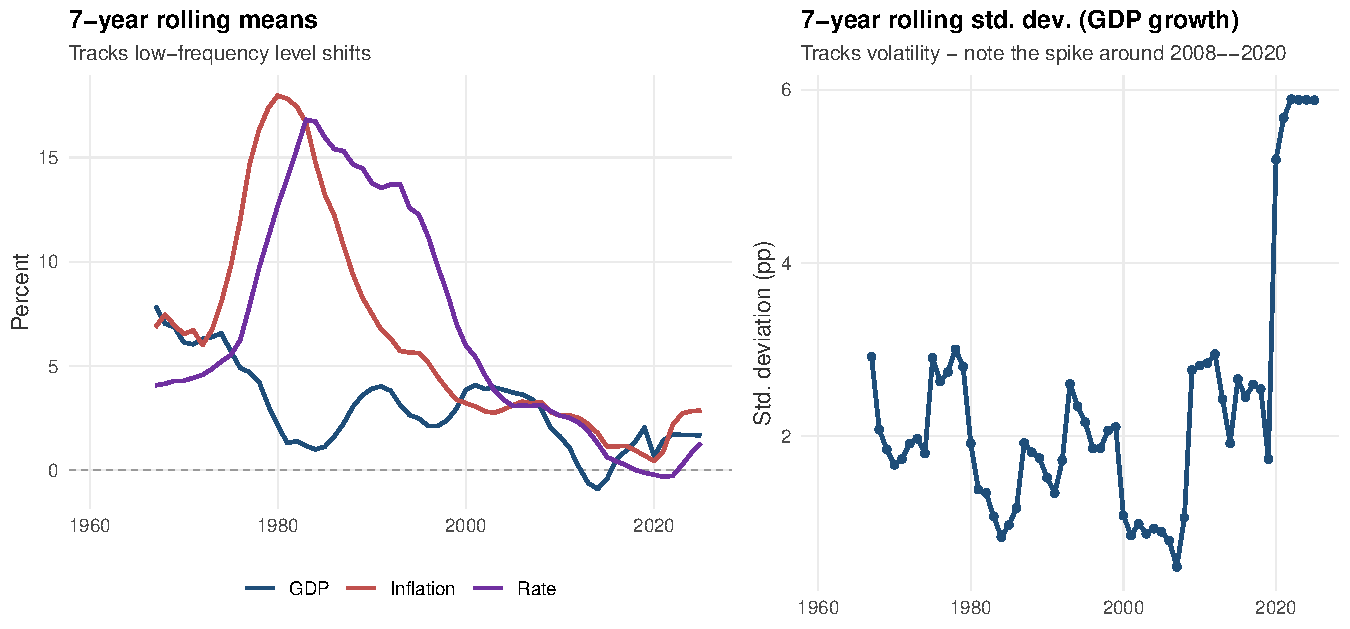
\includegraphics[width=\linewidth]{../output/figures/rolling_stats.pdf}
  \end{column}
  \begin{column}{0.5\textwidth}
    The rolling means highlight the secular decline of inflation and the short rate from the high levels of the 1970s-80s to near-zero readings in the post-2014 ECB window, while average GDP growth shifts down at the GFC. The rolling standard deviation of growth is roughly flat at $\sim$2 pp until 2007, then jumps as the GFC and COVID episodes enter the window; as we will see in Slide~\ref{slide:breaks}, the structural-stability tests examine whether these crisis-period volatility shifts correspond to parameter breaks.
  \end{column}
\end{columns}
\end{block}

\vspace{0.4cm}

\begin{block}{}
\begin{columns}
  \begin{column}{0.5\textwidth}
    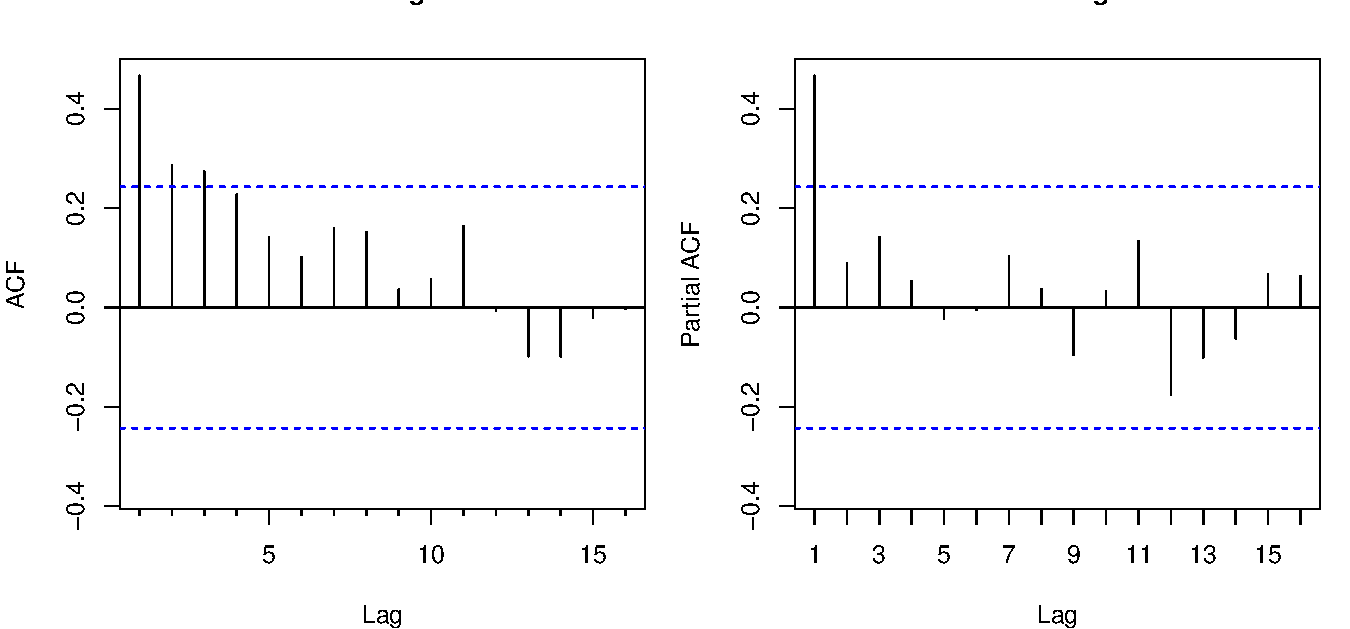
\includegraphics[width=\linewidth]{../output/figures/acf_pacf.pdf}
  \end{column}
  \begin{column}{0.5\textwidth}
    The ACF decays geometrically from a first-order coefficient of approximately 0.45, while the PACF cuts off after the first lag. Both patterns are consistent with a stationary low-order AR process and lend support to the AR(p) and ARIMA candidates considered below. As we will see in Slide~\ref{slide:diagnostics}, the AR(1)/AR(2) specifications also pass residual-autocorrelation checks, supporting the use of low-order autoregressive dynamics.
  \end{column}
\end{columns}
\end{block}
\end{frame}


% ============================================================
% SLIDE 6: Stationarity Tests
% ============================================================
\begin{frame}{(Preliminary) Diagnostic Checks: Stationarity}
\label{slide:stationarity}
\footnotesize
Table~\ref{tab:stationarity} reports ADF (null: unit root) and KPSS (null: level stationarity) tests. We combine the two so that conclusions agree only when both procedures reject in the appropriate direction.

{\footnotesize
\setlength{\tabcolsep}{5pt}
\begin{table}

\caption{\label{tab:stationarity}Unit-root tests, 1961--2025}
\centering
\begin{tabular}[t]{lrrrr}
\toprule
Variable & ADF stat & ADF p-value & KPSS stat & KPSS p-value\\
\midrule
GDP growth & -3.125 & 0.119 & 0.760 & 0.010\\
Inflation & -2.679 & 0.300 & 0.848 & 0.010\\
Short rate & -1.931 & 0.603 & 0.697 & 0.014\\
\bottomrule
\end{tabular}
\end{table}

}

\footnotesize
\begin{itemize}
  \item \textbf{GDP growth shows mixed formal unit-root evidence.} The ADF test does not reject a unit root at the 5\% level, while the KPSS test rejects level stationarity. However, visual inspection and the ACF/PACF pattern suggest mean reversion in GDP growth, and because growth rates are commonly modeled as stationary, we proceed by treating $\Delta y_t$ as approximately I(0), while acknowledging that the formal evidence is not unanimous.

  \item \textbf{Inflation and the short rate} display higher persistence; the KPSS test rejects level stationarity at 5\% for both. Following the macroeconomic literature, we keep the variables in \textit{levels} rather than differencing them, since (a) the Bayesian VAR's Minnesota prior is robust to persistent regressors and (b) cointegration with growth is plausible. As we will see in Slides~\ref{slide:diagnostics}--\ref{slide:forecast-comp}, the diagnostics and forecasting results remain consistent with this modelling choice.
\end{itemize}

\end{frame}


% ============================================================
% SLIDE 7: Cointegration Analysis
% ============================================================
\begin{frame}{(Preliminary) Diagnostic Checks: Cointegration}
\label{slide:cointegration}
\footnotesize

\begin{columns}

  \begin{column}{0.54\textwidth}
    {\fontsize{5.5}{6}\selectfont
    \setlength{\tabcolsep}{2.5pt}
    \setlength{\abovecaptionskip}{2pt}
    \setlength{\belowcaptionskip}{1pt}
    \begin{table}

\caption{\label{tab:engle-granger}Engle--Granger residual-based cointegration test}
\centering
\begin{tabular}[t]{lr}
\toprule
Statistic & Value\\
\midrule
ADF (no constant) on EG residuals & -3.869\\
1\% critical value & -2.600\\
5\% critical value & -1.950\\
10\% critical value & -1.610\\
\bottomrule
\end{tabular}
\end{table}

    \vspace{0.1cm}
    \begin{table}

\caption{\label{tab:johansen}Johansen Trace test (no constant, no trend, K = 2)}
\centering
\begin{tabular}[t]{lrrrr}
\toprule
H0: rank <= r & Trace stat & 10\% & 5\% & 1\%\\
\midrule
r <= 2 & 3.409 & 6.50 & 8.18 & 11.65\\
r <= 1 & 18.533 & 15.66 & 17.95 & 23.52\\
r <= 0 & 37.369 & 28.71 & 31.52 & 37.22\\
\bottomrule
\end{tabular}
\end{table}

    \vspace{0.1cm}
    \begin{table}

\caption{\label{tab:vecm-loadings}Loading (adjustment) matrix $\alpha$ --- rows: equation, columns: ECT}
\centering
\begin{tabular}[t]{lrr}
\toprule
  & ECT1 & ECT2\\
\midrule
GDP growth & -0.485 & 0.006\\
Inflation & 0.122 & 0.002\\
Short rate & 0.013 & 0.240\\
\bottomrule
\end{tabular}
\end{table}

    }
  \end{column}

  \begin{column}{0.46\textwidth}
    \footnotesize
    \begin{itemize}\setlength{\itemsep}{2pt}\setlength{\parskip}{0pt}
      \item The \textbf{Engle--Granger} ADF on the residuals of the static regression $\Delta y_t = \beta_0 + \beta_1 \pi_t + \beta_2 i_t + u_t$ rejects the unit-root null ($-3.869 < -1.950$), single-equation evidence for cointegration among the three series.

      \item The \textbf{Johansen Trace} test selects rank $r=2$ at 5\%: $r=0$ is clearly rejected and $r \leq 1$ marginally so ($18.53$ vs.\ $17.95$), while $r \leq 2$ is not. As $\Delta y_t$ is itself $I(0)$, one relation (ECT1) essentially reflects its own stationarity, while ECT2 is a genuine long-run link, $\pi_t - 0.74\,i_t$, between inflation and the short rate.

      \item The \textbf{loading matrix} $\alpha$ shows adjustment to ECT1 concentrated in the GDP-growth equation ($\approx -0.49$, mean reversion of growth) and adjustment to ECT2 concentrated in the interest-rate equation ($\approx 0.24$): the empirical counterpart of a monetary-policy reaction function.
    \end{itemize}
  \end{column}

\end{columns}

\end{frame}


% ============================================================
% SLIDE 8: Model Specifications
% ============================================================
\subsection{Model Specification}
\begin{frame}{Diagnostic Checks: Model Specifications}
\label{slide:models}
\small

\begin{columns}
  \begin{column}{0.54\textwidth}
    {\fontsize{5}{5.5}\selectfont
    \setlength{\tabcolsep}{2.5pt}
    \setlength{\abovecaptionskip}{1pt}
    \setlength{\belowcaptionskip}{1pt}
    \begin{table}

\caption{\label{tab:ar-arima-models}AR(p) information criteria}
\centering
\begin{tabular}[t]{rrr}
\toprule
p & AIC & BIC\\
\midrule
0 & 348.85 & 353.20\\
1 & 332.79 & 339.31\\
2 & 333.87 & 342.57\\
3 & 333.56 & 344.43\\
4 & 335.36 & 348.41\\
\addlinespace
5 & 337.35 & 352.57\\
\bottomrule
\end{tabular}
\end{table}

    \vspace{0.1cm}
    \begin{table}

\caption{\label{tab:ar2-coef}AR(2): coefficient estimates}
\centering
\begin{tabular}[t]{lrr}
\toprule
term & estimate & std.error\\
\midrule
ar1 & 0.463 & 0.125\\
ar2 & 0.124 & 0.129\\
intercept & 3.442 & 0.875\\
\bottomrule
\end{tabular}
\end{table}

    \vspace{0.1cm}
    \begin{table}

\caption{\label{tab:var-summary}VAR(2): equation for GDP growth}
\centering
\begin{tabular}[t]{lrrrr}
\toprule
term & estimate & std.error & statistic & p.value\\
\midrule
GDP\_Growth.l1 & 0.379 & 0.135 & 2.802 & 0.007\\
Inflation.l1 & 0.039 & 0.161 & 0.243 & 0.809\\
Interest\_Rate.l1 & -0.218 & 0.243 & -0.894 & 0.375\\
GDP\_Growth.l2 & 0.119 & 0.124 & 0.966 & 0.338\\
Inflation.l2 & -0.040 & 0.173 & -0.230 & 0.819\\
\addlinespace
Interest\_Rate.l2 & 0.199 & 0.218 & 0.916 & 0.364\\
const & 1.540 & 0.738 & 2.085 & 0.042\\
\bottomrule
\end{tabular}
\end{table}

    }
  \end{column}

  \begin{column}{0.46\textwidth}
    \footnotesize
    Four models are compared: two univariate (AR dynamics only) and two multivariate (the VAR/BVAR above, exploiting the joint dynamics of $\mathbf{x}_t=(\Delta y_t,\,\pi_t,\,i_t)^{\!\top}$):
    \begin{itemize}\setlength{\itemsep}{3pt}\setlength{\parskip}{0pt}
      \item Both AIC and BIC select an \textbf{AR(1)}; the AR(2) has a small in-sample penalty but matches the assignment specification. \texttt{auto.arima} with BIC confirms ARIMA(1,0,0) with non-zero mean.

      \item All four VAR criteria select a single lag; we estimate the \textbf{VAR(2)} as required by the brief. With 65 observations and 21 parameters, the unrestricted OLS VAR pays a large variance penalty.

      \item We treat the \textbf{BVAR(2)} as our preferred model on a priori grounds (favourable small-sample properties via Minnesota shrinkage) and confirm it ex post via diagnostics and the forecast horse race (Slides~\ref{slide:forecast-eval}--\ref{slide:forecast-comp}).
    \end{itemize}
  \end{column}
\end{columns}

\end{frame}


% ============================================================
% SLIDE 9: Optimal Model Specification
% ============================================================
\begin{frame}{Optimal Model Specification: Why a BVAR?}
\label{slide:bvar}

\textbf{\footnotesize Why a Bayesian Vector Autoregression?}

\scriptsize
\begin{enumerate}
  \item \textbf{Captures simultaneous dynamics across the New-Keynesian triplet}\\
        The triple $(\Delta y,\,\pi,\,i)$ spans the canonical NK three-equation system: aggregate demand, an inflation-augmented Phillips curve, and a monetary-policy reaction function. For Spain, a price-taker in EMU since 1999, the VAR traces the (one-way) transmission of euro-area monetary policy to domestic activity without imposing (often violated) exogeneity assumptions. The cointegration evidence (Slide~\ref{slide:cointegration}) further supports this triplet as economically meaningful.

  \item \textbf{Bayesian shrinkage addresses the small-sample problem}\\
        With only 65 annual observations and 21 reduced-form parameters, the unrestricted OLS VAR pays a steep variance penalty. The Minnesota prior anchors the posterior toward a parsimonious random-walk benchmark, exploiting two stylised facts: (i) own lags carry most predictive content; (ii) higher-order lags add little beyond noise.
        
        As we will see in Slides~\ref{slide:forecast-eval}--\ref{slide:forecast-comp}, this bias--variance trade-off is confirmed ex post.

  \item \textbf{Rich policy diagnostics}\\
        Impulse-response functions (Slide~\ref{slide:granger-irf}) show that a 1\,$\sigma$ positive interest-rate shock reduces GDP growth over 1--3 years, measuring the size of the monetary policy pass-through. The BVAR(2) also achieves well-calibrated 90\% predictive intervals (empirical coverage 80\%) compared with the over-confident unrestricted VAR(2) (Slide~\ref{slide:forecast-comp}).

  \item \textbf{Structural-break evidence motivates robustness checks, but not a more complex model}\\
        As we will see in Slides~\ref{slide:breaks}--\ref{slide:breaks-interp}, the structural-break tests indicate some instability: fixed-date Chow tests reject parameter constancy in 1973, 2008, and 2020, while unknown-date tests point to a late-sample break around 2014–2015. However, with only 65 annual observations, split-sample, dummy-rich, or time-varying-parameter specifications would be difficult to estimate reliably. We therefore keep a single time-invariant benchmark model, but interpret it cautiously and report forecast robustness with and without the 2020 COVID observation (Slide~\ref{slide:forecast-comp}).
\end{enumerate}

\end{frame}


% ============================================================
% SLIDE 10: Structural Stability & Breakpoint Tests
% ============================================================
\begin{frame}{Structural Stability: Breakpoint Tests}
\label{slide:breaks}
\footnotesize

\begin{columns}
  \begin{column}{0.58\textwidth}
    {\fontsize{5.5}{6}\selectfont
    \setlength{\tabcolsep}{2.5pt}
    \setlength{\abovecaptionskip}{2pt}
    \setlength{\belowcaptionskip}{1pt}
    \begin{table}

\caption{\label{tab:chow-tests}Chow F-tests for parameter constancy in the AR(2) for GDP growth}
\centering
\begin{tabular}[t]{lrlrr}
\toprule
Test & Break year & Event & F-statistic & p-value\\
\midrule
CH1 & 1973 & Oil shock \& Bretton-Woods break-up & 3.118 & 0.033\\
CH2 & 1986 & EEC accession & 1.423 & 0.246\\
CH3 & 2008 & Global financial crisis & 4.266 & 0.009\\
CH4 & 2020 & COVID-19 pandemic & 7.047 & 0.000\\
\bottomrule
\end{tabular}
\end{table}

    \vspace{0.1cm}
    \begin{table}

\caption{\label{tab:unknown-breaks}Unknown-date structural-break tests}
\centering
\begin{tabular}[t]{llll}
\toprule
Test & Statistic & Break date(s) & p-value\\
\midrule
Quandt--Andrews sup-F & 18.54 & 2015 & 0.007\\
Bai--Perron (BIC-optimal m) & m = 1 & 2014 & —\\
\bottomrule
\end{tabular}
\end{table}

    }
  \end{column}

  \begin{column}{0.42\textwidth}
    \scriptsize
    \begin{itemize}
      \item \textbf{CH1 (1973)} rejects only marginally ($p=0.033$), whereas \textbf{CH3 (2008)} rejects more firmly ($p=0.009$, significant at 1\%); still, the evidence for a lasting regime change is weaker than for COVID, and these may reflect transitory volatility spikes rather than a structural shift in the AR parameters.
      \item \textbf{CH2 (1986)} does not reject parameter constancy, suggesting the EEC accession was absorbed without disrupting the AR(2) dynamics of Spanish GDP growth.
      \item \textbf{CH4 (2020)} is decisively rejected ($F=7.047$, $p\approx 0$): the COVID contraction is an event of a different magnitude that the linear model cannot accommodate.
      \item The \textbf{Quandt--Andrews} sup-$F$ test locates the most likely unknown break near 2015 (in the expanding-window sense) and rejects stability at 5\%. The \textbf{Bai--Perron} procedure identifies 2014 as the single BIC-optimal break, both suggesting broader late-sample instability, possibly related to the post-euro-crisis recovery or low-rate environment.
    \end{itemize}
  \end{column}
\end{columns}

\end{frame}


% ============================================================
% SLIDE 11: Breakpoint Interpretation & Visual Evidence
% ============================================================
\begin{frame}{Breakpoint Analysis: Interpretation \& Visual Evidence}
\label{slide:breaks-interp}

\begin{columns}

  \begin{column}{0.55\textwidth}
    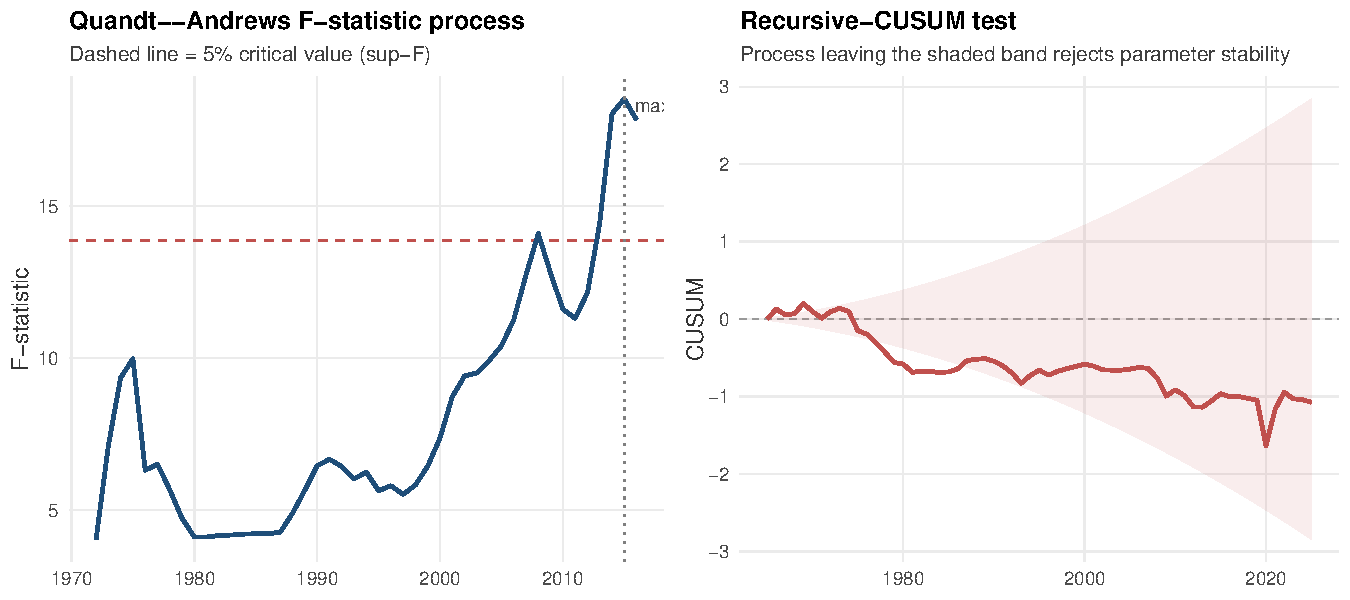
\includegraphics[width=\linewidth]{../output/figures/qlr_cusum_plot.pdf}
    \scriptsize
    The CUSUM process drifts but largely stays inside the 5\% confidence band until the very end of the sample, consistent with a \textit{single late break} rather than systematic structural change throughout. The QLR/CUSUM evidence points to late-sample instability. The fixed-date Chow test strongly detects the 2020 COVID shock, while the unknown-date tests select 2014–2015.
  \end{column}

  \begin{column}{0.45\textwidth}
    \scriptsize
    \textbf{Two practical implications:}\\[0.3em]
    \textbf{1. Sample retention.} Because the pre-2020 dynamics appear relatively stable (CH2 for EEC accession not rejected; CH1 and CH3 only marginally), we keep the \textbf{full 1961--2025 sample} to estimate all models. Splitting the sample would discard relevant high-inflation and high-growth observations without improving fit.\\[0.3em]
    \textbf{2. COVID treatment.} The 2020 observation is a \textbf{one-off exogenous shock} rather than a regime change in the parameter vector. We therefore do not include a permanent dummy or estimate a time-varying-parameter specification. Instead we (i) report forecast accuracy with and without 2020 in the evaluation window and (ii) note that the Minnesota prior of the BVAR naturally absorbs such large innovations without over-parameterising the model (Slide~\ref{slide:forecast-comp}).\\[0.3em]
    The AR(2) coefficients are not stable enough to ignore break evidence entirely: 1973 and 2008 reject parameter constancy, and 2020 is a clear outlier. However, the evidence is not sufficient, given the short sample, to justify estimating separate regimes.
  \end{column}

\end{columns}

\end{frame}


% ============================================================
% SLIDE 12: Diagnostic Checks
% ============================================================
\begin{frame}{Diagnostic Checks}
\label{slide:diagnostics}
\footnotesize

\begin{columns}
  \begin{column}{0.55\textwidth}
    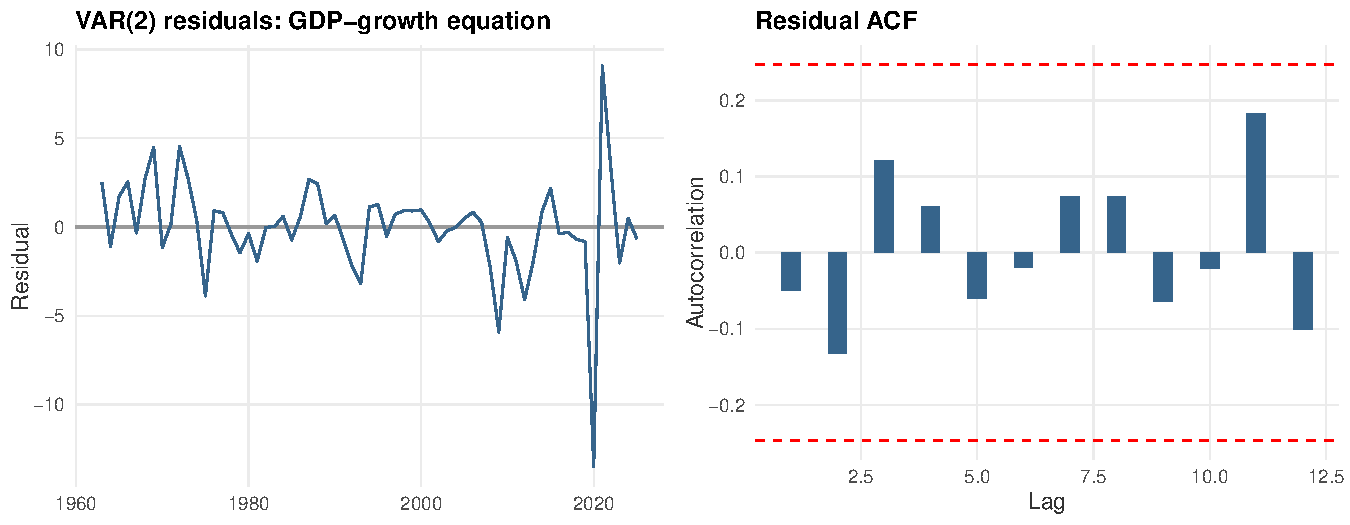
\includegraphics[width=\linewidth]{../output/figures/residual_plot.pdf}
    

    {\fontsize{4.8}{5.3}\selectfont
    \setlength{\tabcolsep}{1.2pt}
    \setlength{\abovecaptionskip}{1pt}
    \setlength{\belowcaptionskip}{1pt}
    \begin{table}

\caption{\label{tab:diagnostics}VAR(2) residual diagnostics}
\centering
\begin{tabular}[t]{lrrl}
\toprule
Test & Statistic & p-value & H0\\
\midrule
Portmanteau (residual autocorrelation) & 57.478 & 0.348 & No serial correlation up to lag 8\\
Jarque--Bera (normality, multivariate) & 224.640 & 0.000 & Normal residuals\\
Multivariate ARCH (heteroskedasticity) & 172.998 & 0.050 & No ARCH effects up to lag 4\\
\bottomrule
\end{tabular}
\end{table}

    }
  \end{column}

  \begin{column}{0.45\textwidth}
    \scriptsize
    The \textbf{Portmanteau} test does not reject no residual autocorrelation ($p=0.348$): two lags adequately capture the joint dynamics. The \textbf{Jarque--Bera} test rejects normality, unsurprising given the COVID-19 outlier; this matters for finite-sample inference but does not affect point-forecast consistency. The \textbf{ARCH} test is borderline ($p=0.050$), providing only marginal evidence of conditional heteroskedasticity and not rejecting homoskedasticity at the 5\% level. The residuals fluctuate around zero with no visible pattern beyond the COVID spike; the residual ACF lies inside the 95\% confidence bands at all displayed lags.

    {\fontsize{5}{5.5}\selectfont
    \setlength{\tabcolsep}{1.5pt}
    \setlength{\abovecaptionskip}{1pt}
    \setlength{\belowcaptionskip}{1pt}
    \begin{table}

\caption{\label{tab:stability}Moduli of the companion-matrix roots}
\centering
\begin{tabular}[t]{rr}
\toprule
Root & Modulus\\
\midrule
1 & 0.9093\\
2 & 0.9093\\
3 & 0.6019\\
4 & 0.2276\\
5 & 0.2271\\
\addlinespace
6 & 0.2271\\
\bottomrule
\end{tabular}
\end{table}

    }
    \vspace{0.05cm}
    \scriptsize All roots lie strictly inside the unit circle: the VAR(2) is covariance-stationary.

    \vspace{0.15cm}
  \end{column}
\end{columns}

\end{frame}


% ============================================================
% SLIDE 13: Economic Hypotheses: Granger Causality & IRFs
% ============================================================
\begin{frame}{Economic Hypotheses: Granger Causality \& Impulse Responses}
\label{slide:granger-irf}
\footnotesize

\begin{columns}
  \begin{column}{0.55\textwidth}
    {\fontsize{5.5}{6}\selectfont
    \setlength{\tabcolsep}{2.5pt}
    \setlength{\abovecaptionskip}{2pt}
    \setlength{\belowcaptionskip}{1pt}
    \begin{table}

\caption{\label{tab:granger}Block Granger-causality tests}
\centering
\begin{tabular}[t]{lrr}
\toprule
Null hypothesis & F-statistic & p-value\\
\midrule
Interest rate does not Granger-cause (GDP, infl) & 0.541 & 0.706\\
Inflation does not Granger-cause (GDP, rate) & 5.301 & 0.000\\
GDP growth does not Granger-cause (infl, rate) & 0.481 & 0.750\\
\bottomrule
\end{tabular}
\end{table}

    }
    \scriptsize
    The pattern matches the textbook small monetary VAR. \textbf{Inflation} Granger-causes the joint block ($\Delta y + i$) at conventional levels, consistent with both a Phillips-curve-type relationship and a policy-reaction function. By contrast, the short-rate and GDP-growth nulls are not rejected, suggesting limited predictive causality from these variables in the annual sample. We must note that with only 65 annual observations, the tests have limited power.
  \end{column}

  \begin{column}{0.45\textwidth}
    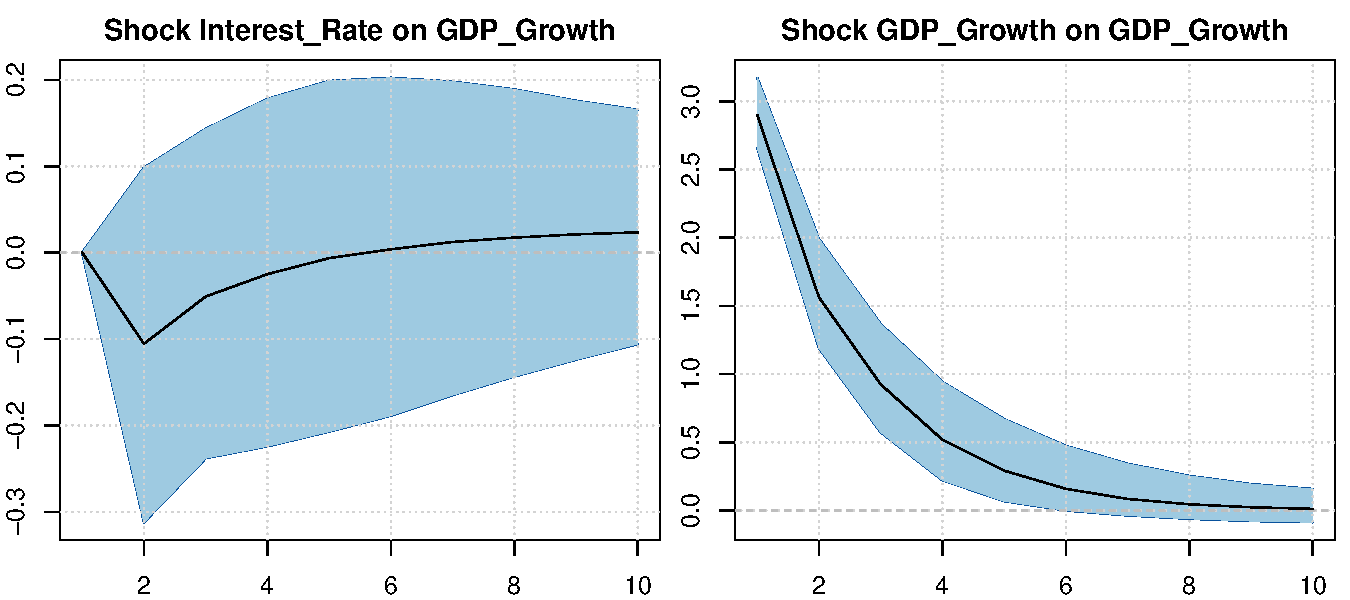
\includegraphics[width=\linewidth]{../output/figures/bvar_irf.pdf}
    \scriptsize
    BVAR(2) impulse responses. The point estimate of the response of GDP growth to a 1\,$\sigma$ positive interest-rate shock is \textbf{negative on impact and over the first three years}, consistent with the standard monetary policy mechanism, although the 84\% credible band straddles zero, another reflection of the limited identification afforded by an annual sample. The own-shock response of GDP growth decays smoothly toward zero, consistent with the AR(1)-like behaviour of the series.
  \end{column}
\end{columns}

\end{frame}


% ============================================================
% SLIDE 14: Forecasting Evaluation — Point Forecast
% ============================================================
\subsection{Forecast Evaluation}
\begin{frame}{One-step-ahead Forecasting Evaluation}\label{slide:forecast-eval}
\small

\begin{figure}
  \centering
  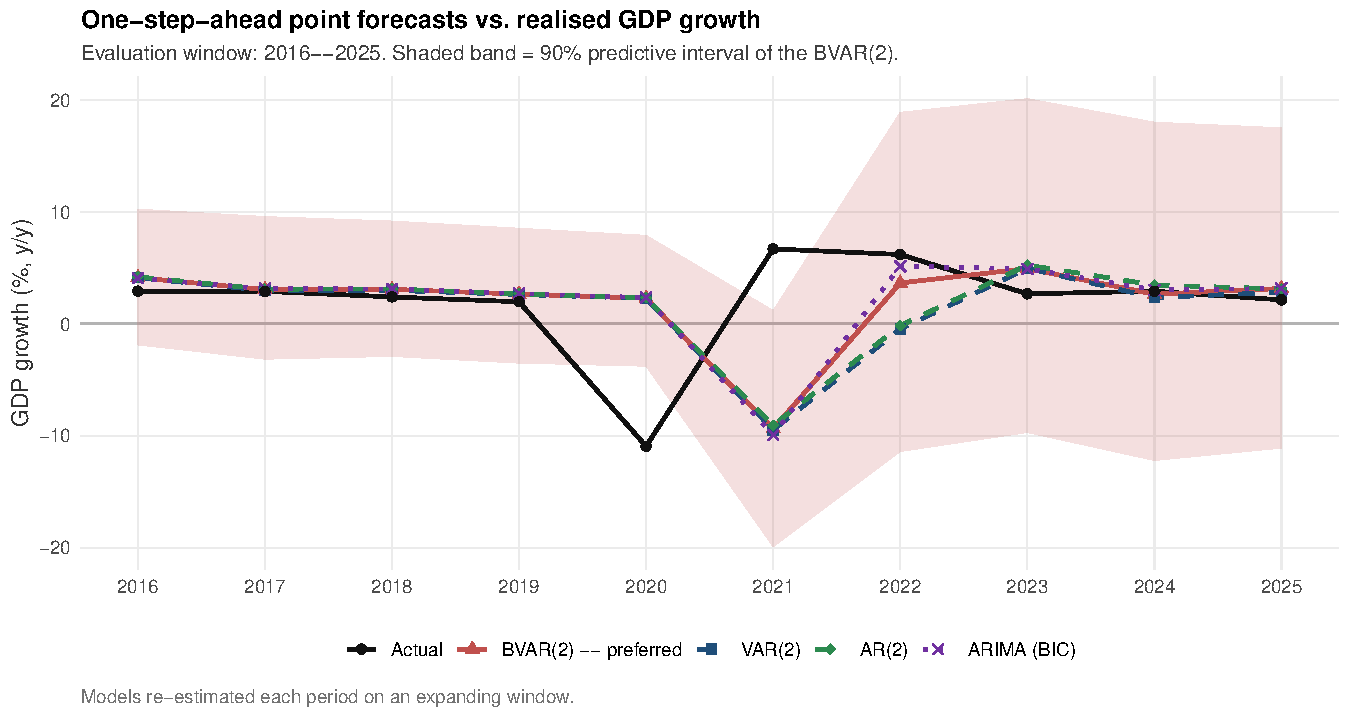
\includegraphics[width=0.72\linewidth]{../output/figures/forecast_plot.pdf}
\end{figure}

\vspace{0.05cm}

{\footnotesize
\setlength{\tabcolsep}{4pt}
\begin{table}

\caption{\label{tab:forecast_acc}1-step-ahead forecast accuracy (last 10 years)}
\centering
\begin{tabular}[t]{lrrrr}
\toprule
Model & RMSE & MAE & ME & Theil's U\\
\midrule
BVAR(2) -- preferred & 6.693 & 3.809 & 0.034 & 0.954\\
ARIMA (BIC) & 6.794 & 3.713 & 0.181 & 0.968\\
AR(2) & 6.890 & 4.236 & -0.184 & 0.982\\
VAR(2) & 6.987 & 4.207 & -0.471 & 0.996\\
\bottomrule
\end{tabular}
\end{table}

}

\end{frame}


% ============================================================
% SLIDE 15: Forecast Comparison
% ============================================================
\subsection{Forecast Comparison}
\begin{frame}{Forecast Comparison}\label{slide:forecast-comp}

\small

\begin{columns}
  \begin{column}{0.62\textwidth}
\vspace{-0.2cm}
    {\fontsize{5}{5.5}\selectfont
    \setlength{\tabcolsep}{1.2pt}
    \setlength{\abovecaptionskip}{1pt}
    \setlength{\belowcaptionskip}{1pt}
    \begin{table}

\caption{\label{tab:dm-tests}Diebold--Mariano tests of equal predictive accuracy (squared-loss)}
\centering
\begin{tabular}[t]{lrr}
\toprule
Comparison & DM stat & p-value\\
\midrule
BVAR vs VAR(2) & -1.066 & 0.314\\
BVAR vs AR(2) & -0.739 & 0.478\\
BVAR vs ARIMA & -0.713 & 0.494\\
AR(2) vs VAR(2) & -0.959 & 0.363\\
\bottomrule
\end{tabular}
\end{table}

    \vspace{0.1cm}
    \begin{table}

\caption{\label{tab:forecast-coverage}Calibration of one-step-ahead 90\% predictive intervals}
\centering
\begin{tabular}[t]{lrr}
\toprule
Model & Empirical coverage of 90\% PI & Average PI width (pp)\\
\midrule
BVAR(2) -- preferred & 0.8 & 20.066\\
VAR(2) & 0.7 & 7.885\\
AR(2) & 0.7 & 8.262\\
ARIMA (BIC) & 0.8 & 8.243\\
\bottomrule
\end{tabular}
\end{table}

    \vspace{0.1cm}
    \begin{table}

\caption{\label{tab:forecast-accuracy-ex-covid}Forecast accuracy excluding the 2020 COVID outlier}
\centering
\begin{tabular}[t]{lrr}
\toprule
Model & RMSE & MAE\\
\midrule
BVAR(2) & 5.510 & 2.764\\
ARIMA (BIC) & 5.633 & 2.651\\
AR(2) & 5.762 & 3.233\\
VAR(2) & 5.904 & 3.207\\
\bottomrule
\end{tabular}
\end{table}

    }
  \end{column}

  \begin{column}{0.38\textwidth}
    \tiny
    \begin{itemize}\setlength{\itemsep}{2pt}\setlength{\parskip}{0pt}
      \item \textbf{Point accuracy.} The BVAR(2) attains the lowest RMSE and 2nd lowest MAE in the full evaluation window, with the AR(2) and ARIMA following closely. The unrestricted VAR(2) is the worst performer, consistent with its larger small-sample estimation variance. Excluding the 2020 observation reduces all RMSEs by roughly 17\% on average but leaves the ranking unchanged: shrinkage continues to dominate.

      \item \textbf{Statistical significance.} All DM statistics are negative, pointing in the same direction as the RMSE ranking, but the 10-year window is too short to reject equal predictive accuracy ($p > 0.05$). The accuracy gains are economically meaningful but statistically inconclusive given the short evaluation window.

      \item \textbf{Interval calibration.} Theil's U lies below 1 for every model, so all four out-perform a naive random-walk benchmark. The BVAR(2) and ARIMA attain the closest-to-nominal 90\% coverage (80\%), whereas VAR(2) and AR(2) under-cover (70\%). Crucially, the BVAR(2) reaches its coverage with honestly wide intervals ($\approx 20$ pp), while the VAR(2)/AR(2) bands ($\approx 8$ pp) are over-confident rather than sharper. The combined evidence---lowest RMSE, 2nd-lowest MAE, DM statistics that all point the same way, and well-calibrated intervals---\textbf{substantiates the a priori preference for the BVAR(2)}.
    \end{itemize}
  \end{column}
\end{columns}

\end{frame}

\begin{frame}{References and LLM Declaration}
\label{slide:refs}
\scriptsize

\textbf{References}

\begin{itemize}
    \item Bańbura, M., Giannone, D., \& Reichlin, L. (2010). Large Bayesian vector autoregressions. \textit{Journal of Applied Econometrics}, 25(1), 71--92.
    \item Litterman, R. B. (1986). Forecasting with Bayesian vector autoregressions - five years of experience. \textit{Journal of Business \& Economic Statistics}, 4(1), 25--38.
    \item Müller, K., Schularick, M., \& Trebesch, C. (2024). \textit{The Global Macro Database} (Spain country file).
\end{itemize}

\vspace{0.25cm}

\textbf{Use of Large Language Models}

Per the assignment guidelines, we declare that an LLM (Anthropic Claude) was used as an assistant for:
(i) editing and polishing the written exposition;
(ii) helping organise the presentation of empirical results; and
(iii) cleaning up and reorganising R scripts. All analytical decisions, numerical results, and substantive conclusions were independently reviewed and confirmed by the authors.

\end{frame}

\end{document}
